\documentclass[twoside, a4paper, 12pt]{article}

%Package Settings

\usepackage[utf8]{inputenc}
\usepackage[margin=2.5cm, includefoot]{geometry}
\usepackage{setspace}
\doublespacing
\usepackage[backend=biber,authordate-trad]{biblatex-chicago}
\addbibresource{Refs.bib}
\usepackage{graphicx}
\usepackage{csquotes}
\usepackage{fancyhdr}
\usepackage{titling}
\usepackage[hidelinks]{hyperref}
\usepackage{wrapfig}
\usepackage{float}
\usepackage{caption}
\usepackage{soul}

% Page Style Stuff
\fancypagestyle{plain}{
  \fancyhf{}
  \renewcommand{\headrulewidth}{0.1pt}
  \renewcommand{\footrulewidth}{0.4pt}
  \fancyfoot[LE,RO]{\theauthor}
  \fancyfoot[C]{\thetitle}
  \fancyfoot[RE,LO]{Page \thepage}
}

% Title Formatting
\title{Greek Battle Strategy \\ And Its Victory Over Persia}

\author{Luke Hedt}
\date{\today}

\setul{}{0.2pt}

% Allows for sourcing images
\newcommand{\source}[1]{\caption*{Source: {#1}} }

% Handy Citation Notes for later:
% \footcite[200]{morris_powell_2010} %To add page numbers to citations
% \blockquote{} % If you plan to quote a huge section of Herodotus

\begin{document}

\pagenumbering{Alph}
\begin{titlepage}
    \centering
    
\includegraphics[width=0.25\textwidth]{UniLogo.png}\par\vspace{1cm}
    {\scshape\Large THE UNIVERSITY OF MELBOURNE \\
              \large ANCW20022 Ancient Greece: \\
              History and Archaeology Essay\par}
    \vspace{1.5cm}
    {\Huge \thetitle \par}
    \vfill

% Bottom of the page
    {\Large\itshape \theauthor \hspace{1em} -- \hspace{1em} 832153 \par}
    \vspace{1.5cm}
    {\Large \today}
\end{titlepage}
% Format first page correctly.
\pagestyle{plain}
\pagenumbering{arabic}

The early fifth century BC was a pivotal period in the formation of the Hellenic
identity, marking the decisive point between the period of \emph{p{\'o}leis} Greece
and the true Hellenic period. The cornerstone of this identity formation
was the defeat of Persia in the Greco-Persian Wars, beginning in 499 BC
with the Ionian Revolt. But what brought about the defeat of Persia? What tactics
were the Greeks employing in the period that brought about their victories?
This essay will attempt to address these questions, discussing how their
strategies and arms and armour were instrumental in the defeat of Persia
in the Greco-Persian Wars and
Carthage in the First Sicilian War.

\par\vspace{1em}

\begin{wrapfigure}{R}{0.4\textwidth}
  \centering
  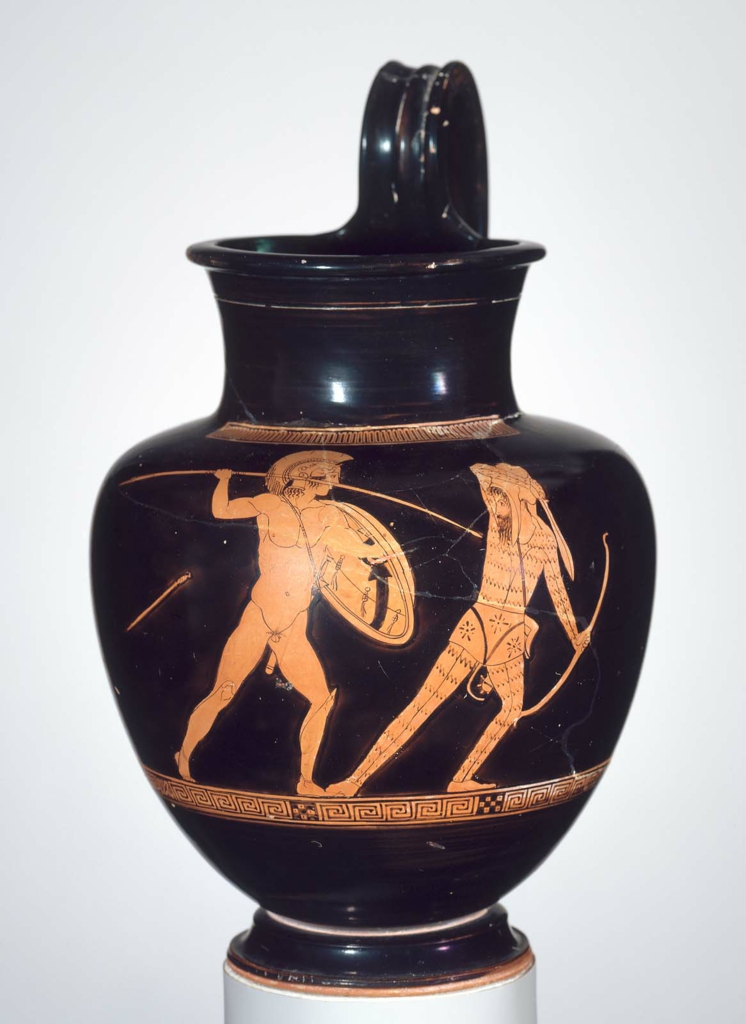
\includegraphics[width=\linewidth]{HopliteArcher.jpg}
  \captionsetup{justification=raggedleft}
  \caption{\ul{ Pottery art of a Greek Hoplite attacking a Persian Archer, circa 450 BC.}}
  \source{\cite{MFABoston_2017_hoplite}}
  \label{img:HopliteArcher}
\end{wrapfigure}

The Greek City States were not a cohesive unit at the outbreak of the fifth century
BC as we tend to think of them today. Rather each urban centre (the
\emph{polis}) controlled
the land around it, and considered itself a separate (and usually superior, especially
in the case of Athens)
entity to the other cities that would now be considered Greek. A person's city of
origin was usually considered more important than their `Greekness.' It was
a more prominent identifier, to be from Athens or Halicarnassus
as in the case of Herodotus, than to be Greek prior to the
Greco-Persian Wars.
\footcite{kim_grecopersia_2017}
However, most of the Greek city states often equipped
themselves rather similarly, copying the armour style of Sparta, the most
effective fighting force in the locality.
The Greek armies are famous for their \emph{hoplite} infantry units, heavily
armoured spear infantry with a distinctive large wooden shield. The shield is
the most important common component, appearing first with the
identifiable double handle in pottery art
circa 700 BC.\footnotemark
The shield was an integral part of infantry kit, being the key defence in battle,
protecting the soldier's front from both the spears and swords of the enemy
infantry, and from arrows from the sky.
Most artistic interpretations of \emph{hoplites} tend to resemble the pottery
style in \textbf{Figure \ref{img:HopliteArcher}}, spear in the overhand
position and the shield protecting the left-hand side of the body.

\par\vspace{1em}

The widely accepted view is that these depictions are in a `heroic' pose, and not
reflective of real spear techniques. An alternative idea exists
that the technique is actually early hoplite tactics and not just a heroic
pose,\footnotemark[\value{footnote}] however the pose has several issues from
a battle perspective.
\footnotetext{\cite[57]{wees_hoplite_bronze}}
Firstly, holding the spear in such a way loses one of the main advantages of a
spear; keeping the enemy a spear's-length away.
To get a balanced spear in the overhand grip, you're required
to keep over half the spear behind your back. Not only do you lose the reach here,
but you're probably going to hit the man behind you in the head because you
can't see what you're doing. It would be far more likely that any weapon held
this way would have a large counterweight on the butt of the spear, keeping it short
and balanced, but such weapons don't appear in art or archaeology. In some Persian
art involving the immortals a small metal ball-weight can be observed, as in
\textbf{Figure \ref{img:ImmortalSusa}},
however it is so small it's probably only to relieve wrist-strain. The
centre of balance on these spears would still be about half way
up the spear. Secondly,
such a hold is very taxing on the biceps. As strong as Greek men may have been
in antiquity, it seems unlikely that anyone could be bothered holding a spear
up for the duration of a fight when you can use your elbow as a lever in
an under-arm grip.

\par\vspace{1em}

Several schools of thought exist regarding the early hoplite formations. The
main two argue the density of formations, based on where the man held his shield.
Victor Davis Hanson argues that the shield implies a tight formation wherein
a solider must rely on his right-hand neighbour's shield for protection, and
that the shield was an adaptation for a more useful dense formation.\footnotemark
\footnotetext{\cite{hanson_keegan_2009}, found through
    \cite[58]{wees_hoplite_bronze}}
Certainly this is quite a possibility for the well trained Spartans, with a
trust built up over a lifetime of training together. However for the less
professional Ionian armies, it seems somewhat less likely that a man would be
willing to trust his life to someone he's barely trained with. Certainly
in the context of the Battle of Marathon, wherein the Athenians
`were sent forth and charged the foreigners at a run,'
\footcite[Book 6.112]{herodotus_1920} Van Wees' argument of the hoplites taking
a more side-on position behind the shield fits much better.
This formation would also require no dependency on your
fellow soldier, \footcite[58]{wees_hoplite_bronze} making it more adaptable to
the one-on-one confrontations pictured in the pottery art.

\par\vspace{1em}

Hoplite armour from here tends to vary a lot more. The hoplites
were usually drawn from the classes that could afford the gear, \footcite[38]{wietzel_wheeler_1970}
so the standing armies may not have always been armoured the same, with gear
missing if it couldn't be purchased. The next main pieces of armour a hoplite
would be wanting were usually their Corinthian helmet (the famous horsehair
ones, though they didn't always have the horsehair) and probably a pair of greaves.
Van Wees argues that due to a limited number of greaves in archaeological finds,
perhaps only a third of hoplites wore them, \footcite[50]{wees_2004} possibly given
that military kit was expensive. Certainly a helmet would have been a priority
over leg armour given how delicate the human head is. Finally, a hoplite would
wear a corselet, bronze body armour held together with leather and bronze banding.
About one in ten hoplites wore the corselet,\footcite{wees_1997} based on
arcaeological findings. As the rarest part of the major
armour parts it was probably the most expensive, and least necessary given the
hoplite would have a shield to keep weapons out of his torso.

\par\vspace{1em}

\begin{wrapfigure}{L}{0.4\textwidth}
  \centering
  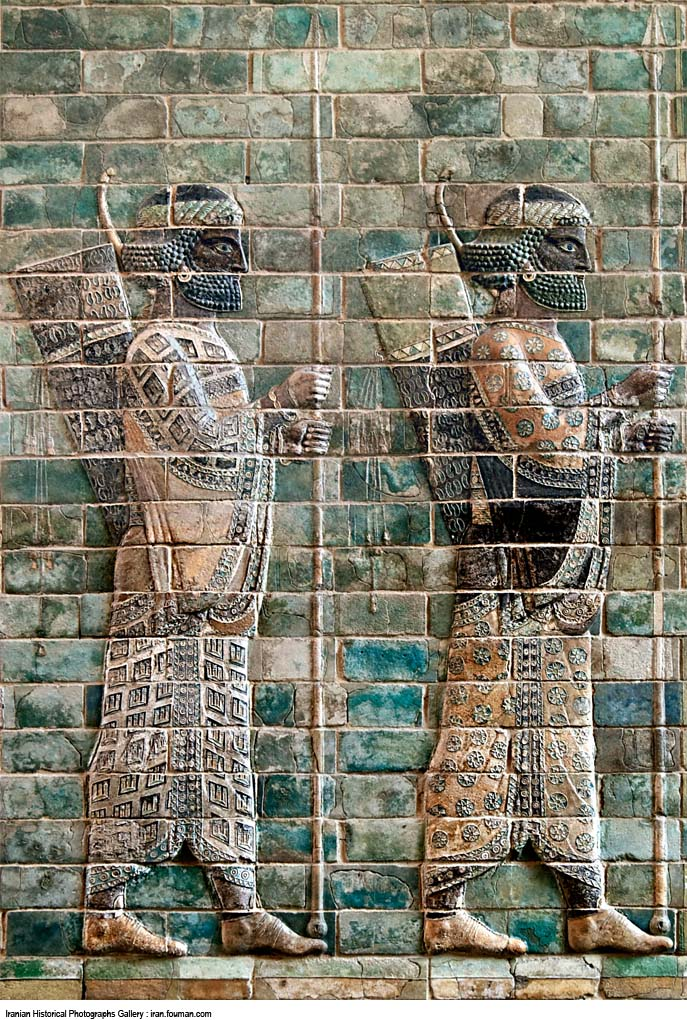
\includegraphics[width=\linewidth]{ImmortalsSusa.jpg}
  \captionsetup{justification=raggedright}
  \caption{\ul{Immortals as depicted in a mural in Susa, circa 510 BC}}
  \source{\emph{Mus\'ee du Louvre}, Paris, \\ via \cite{iranian_historical_photography}}
  \label{img:ImmortalSusa}
\end{wrapfigure}

The Persian Empire was one of the most formidable fighting forces in the world
in the early fifth century BC, having been formed mere decades prior with
Cyrus the Greats' rebellion against the Median Empire. Throughout the
Greco-Persian Wars of the fifth century, it's rather unlikely that the arms
and armament of the Persian military evolved too much, they were after all,
the greatest army on earth in the period. \footcite{kim_grecopersia_2017}
The general consensus for the Persian equipment is somewhat mixed.
Herodotus mentions several times that during the campaigns in Greece that
the Persians lost due to being under-equipped and under-armoured.
`They wore no armour over their clothing, for they fought as it were
naked against men fully armed' \footcite[Book 9.63.2]{herodotus_1920}
Herodotus writes. This particular phrase comes from the account of the battle
of Plataea, near the end of the Greco-Persian War, so it's possible that this
is in reference to a tired, flagging who have lost supplies and are ready
to withdraw. \footcite[267]{charles_bodyarmour_2012}
However Herodotus does reference several types of body armour in his \emph{Histories}.
Charles (and Herodotus to an extent) separates the main types of Persian body armour
into ethnic groups, suggesting that there was a difference between Median,
ethnic Persian and Egyptian cuirasses,
\footcite[Book 1.135]{herodotus_1920}
with the Persian style being an iron
scale type, the Median being some kind of unclear distinction from this, and
the Egyptian being a linen cuirass.\footcite[260-2]{charles_bodyarmour_2012}

\par\vspace{1em}

The enitre Persian Grand army was something of a combination of the militaries
of their conquered nations, as well as various mercenary soldiers. The army had
a good balance of the standard ancient military divisions, archers, infantry
and horsemen. The archers were the first line of attack, lining up behind
shield bearers and firing volleys into the enemy lines, thinning them. Most
of the art surrounding Persian archers pictures them un-armoured with a recurve
bow. Interestingly the infantry unit made famous by Herodotus, the \emph{Immortals},
are often pictured with a bow and a quiver as well as their spear and shield
(for example, see \textbf{Figure \ref{img:ImmortalSusa}}.)

\par\vspace{1em}

In 512 BC, the Greek states were becoming restless with Persian rule. Despite
being somewhat indirect rulers of numerous Greek cities in Ionia, only requiring
a small tax from their subjects, the idea of being beholden to another nation
was insulting to the Greek cities.

\par\vspace{1em}

As a warning to all his satraps(?), Darius had to react to the Ionian
insurrection. A plan to take Athens and subjugate its leaders was formed,
and troops sailed for Greece at once from the Persian heart.

\par\vspace{1em}

A nation resisting Persian subjugation could never stand for long without
becoming the Emperor's target once again, and the Greek states were no
exception. Darius' successor Xerxes would attempt to sack Greece for its worth
and prove that Persia had military dominance in all her Empire. So once again
the Persian's sailed for Greece, landing just North of Thessaly.
Blah Blah Thermopylae.

\par\vspace{1em}

With the Spartans' defeat secured, Xerxes continued marching South for
Athens, intending to burn her, and that he did. The Athenians asked for advice
from Delphi, which was cryptic as ever.
Blah Blah burning Athens, run to the ships.

\par\vspace{1em}

With nothing but the Athenian Navy left, Persia was lead into a trap
by Themistocles in Salamis. Big battle, many sink, much death, win Greece.

\par\vspace{1em}

Plataea and Mycale, ie Persia gets slaughtered against all odds, and
Greece gains a Hellenic identity, naming themselves around Thessaly, where
no battles were fought and nothing really happened except they got some horses
so lol?

\par\vspace{1em}

Sicilian War, Carthage takes on the Sicilian Greeks and gets its arse handed to
it.

\par\vspace{1em}

Overall Greece should have had no chance against the Persians, and the
Carthaginians probably should have been bigger baddies than they were lol.

% Bib page
\newpage
\small{
  \listoffigures
  \printbibliography
}

\end{document}
